\chapter{Implementation}

This chapter covers how each component of the framework was built. It steps through the documentation ingestion pipeline, the two-stage retrieval stack, the provider metadata registry that decouples cloud-specific knowledge from agent logic, the LangGraph graph topology, concurrent state management, per-run model selection, the Next.js user interface, and the evaluation infrastructure.

\section{Data Ingestion and Vector Database Construction}

Factual validation depends on an up-to-date knowledge base of official cloud documentation. The following subsections describe how that documentation is collected, parsed, embedded, and indexed for both AWS and Azure.

\subsection{AWS Documentation Pipeline}

AWS documentation is gathered through a custom Python web scraping pipeline targeting \url{https://docs.aws.amazon.com/}. The pipeline proceeds through four stages:

\begin{itemize}
    \item \textbf{Link extraction:} Using the \texttt{requests} and \texttt{BeautifulSoup} libraries, the scraper traverses the main landing page XML sitemap (\texttt{/en\_us/main-landing-page.xml}) to discover service-specific documentation roots, then filters for developer guides, whitepapers, and API references.
    \item \textbf{PDF discovery:} For each service root the scraper probes multiple subpaths for a \texttt{meta-inf/guide-info.json} metadata file, following HTTP redirects to resolve the canonical direct-download URL for the PDF.
    \item \textbf{Manual supplement:} Services with non-standard documentation layouts (e.g.\ landing pages that do not expose a guide-info endpoint) are identified through manual review and added to a curated supplement list that is merged with the automated output.
    \item \textbf{Storage:} Discovered URLs are deduplicated by their canonical PDF path and written to a structured CSV with metadata columns for service name, documentation type, and source URL, ready for downstream processing.
\end{itemize}

\subsection{Azure Documentation Pipeline}

Unlike AWS, Microsoft hosts its technical documentation openly on GitHub under the \texttt{MicrosoftDocs} organisation. A separate pipeline uses this structure by running \texttt{git sparse-checkout} against the relevant service repositories, pulling only the Markdown files for the required service categories. This approach avoids anti-scraping measures, eliminates HTML-to-text conversion artefacts, and guarantees that the ingested Markdown matches exactly what Microsoft's documentation portal renders.

\subsection{Document Parsing and Chunking}

Raw PDFs (AWS) and Markdown files (Azure) are converted to clean, uniformly formatted Markdown using the Docling toolkit~\cite{docling2025paper, docling2024web}. The Docling parser handles multi-column layouts, embedded tables, and figures; non-vectorisable elements such as images and decorative tables are stripped during a preprocessing pass. The resulting Markdown is split in two stages using LangChain utilities: \texttt{MarkdownHeaderTextSplitter} first divides the document along heading boundaries to preserve section coherence, and \texttt{RecursiveCharacterTextSplitter} then subdivides any sections that exceed the target chunk size. Each chunk retains source URL, service name, and cloud provider as metadata fields, enabling filtered retrieval at query time.

\subsection{Embedding and Indexing}

The \texttt{nomic-embed-text} model, served locally through Ollama~\cite{ollama2024web}, generates dense vector embeddings for each document chunk. On Apple Silicon hardware the embedding computation is accelerated using PyTorch's MPS backend~\cite{apple2024mps}, avoiding the CPU bottleneck for large corpora. Embeddings are stored in provider-scoped ChromaDB collections~\cite{chromadb2024}---a dedicated collection for AWS documentation and a separate collection for Azure---each persisted as an on-disk SQLite store. At application startup, the \texttt{create\_vector\_store} function loads the appropriate collection from disk using the path and collection name resolved from runtime configurations, so no re-embedding is required between runs.

\subsection{Two-Stage Retrieval with Cross-Encoder Reranking}

At query time it is a two-stage retrieval protocol. In the first stage, ChromaDB returns the top $k \times m$ candidates ranked by cosine similarity between the query embedding and stored chunk embeddings, where $m$ is a configurable candidate multiplier (defaulting to 4). In the second stage, when reranking is enabled, FlashRank applies the \texttt{ms-marco-MiniLM-L-12-v2} cross-encoder to score each candidate passage jointly with the query string, and only the top $k$ passages are retained. The cross-encoder's joint attention mechanism captures fine-grained relevance signals---such as the precise configuration context of a cloud service flag---that bi-encoder cosine similarity misses. The \texttt{Ranker} instance is cached in a module-level dictionary keyed by model name, so model weights are loaded once per process rather than per retrieval call.

\section{Provider Metadata Registry}
\label{sec:provider_meta}

A central design principle of the implementation is the strict separation of cloud-provider knowledge from agent and graph logic. All provider-specific information is encapsulated in a frozen \texttt{ProviderMeta} dataclass. The frozen nature of the dataclass prevents accidental mutation during parallel node execution. Each \texttt{ProviderMeta} instance carries the following fields:

\begin{itemize}
    \item \textbf{Domain services:} Maps each architecture domain (compute, network, storage, database) to a comma-separated string of representative services for that provider. For example, the AWS compute entry lists \texttt{EC2, Lambda, ECS, EKS, Auto Scaling}. These strings are injected directly into supervisor and domain architect system prompts, so agents inherently reason about provider-appropriate services without any conditional logic in the agent code itself.
    \item \textbf{Validation checks:} Maps each domain to a numbered checklist of validation criteria. For instance, the AWS network domain specifies checks for VPC CIDR configuration, security group rules, load balancer setup, DNS, and routing correctness. Domain validator agents receive this checklist as part of their system prompt, ensuring consistent and comprehensive validation across runs.
    \item \textbf{IaC resource hints:} Maps each domain to canonical Infrastructure-as-Code resource type identifiers. The AWS compute domain, for example, maps to \texttt{aws\_instance}, \texttt{aws\_lambda\_function}, \texttt{aws\_ecs\_service}, \texttt{aws\_eks\_cluster}, and related Terraform resource types. These hints are injected into the final architecture generator prompt so that the output document can include concrete IaC stubs.
    \item \textbf{Supported IaC formats:} A tuple declaring which IaC dialects the provider supports, such as \texttt{("terraform", "cloudformation")} for AWS or \texttt{("terraform", "bicep")} for Azure.
    \item \textbf{RAG tool description:} A provider-scoped natural-language description bound to the RAG search tool. This text informs the LLM which documentation corpus the tool interrogates, preventing cross-provider retrieval confusion.
\end{itemize}

Two instances, \texttt{AWS\_META} and \texttt{AZURE\_META}, are registered in the common dictionary. The \texttt{ArchitectureService} resolves the active provider at startup from the \texttt{provider\_mode} configuration setting (\texttt{"aws"}, \texttt{"azure"}, or \texttt{"both"}). Extending the framework to Google Cloud Platform requires only defining a \texttt{GCP\_META} entry and adding it to the registry; no agent, graph, or tool code requires modification.

\section{Agentic Workflow and Graph Orchestration}

The system is implemented as a cyclic multi-agent graph managed by LangGraph~\cite{langgraph2024docs}. The complete orchestration, including conditional feedback edges, is visualised in the graph structure generated by LangGraph Studio, as shown in Figure~\ref{fig:langgraph}.

\begin{figure}[H]
\centering
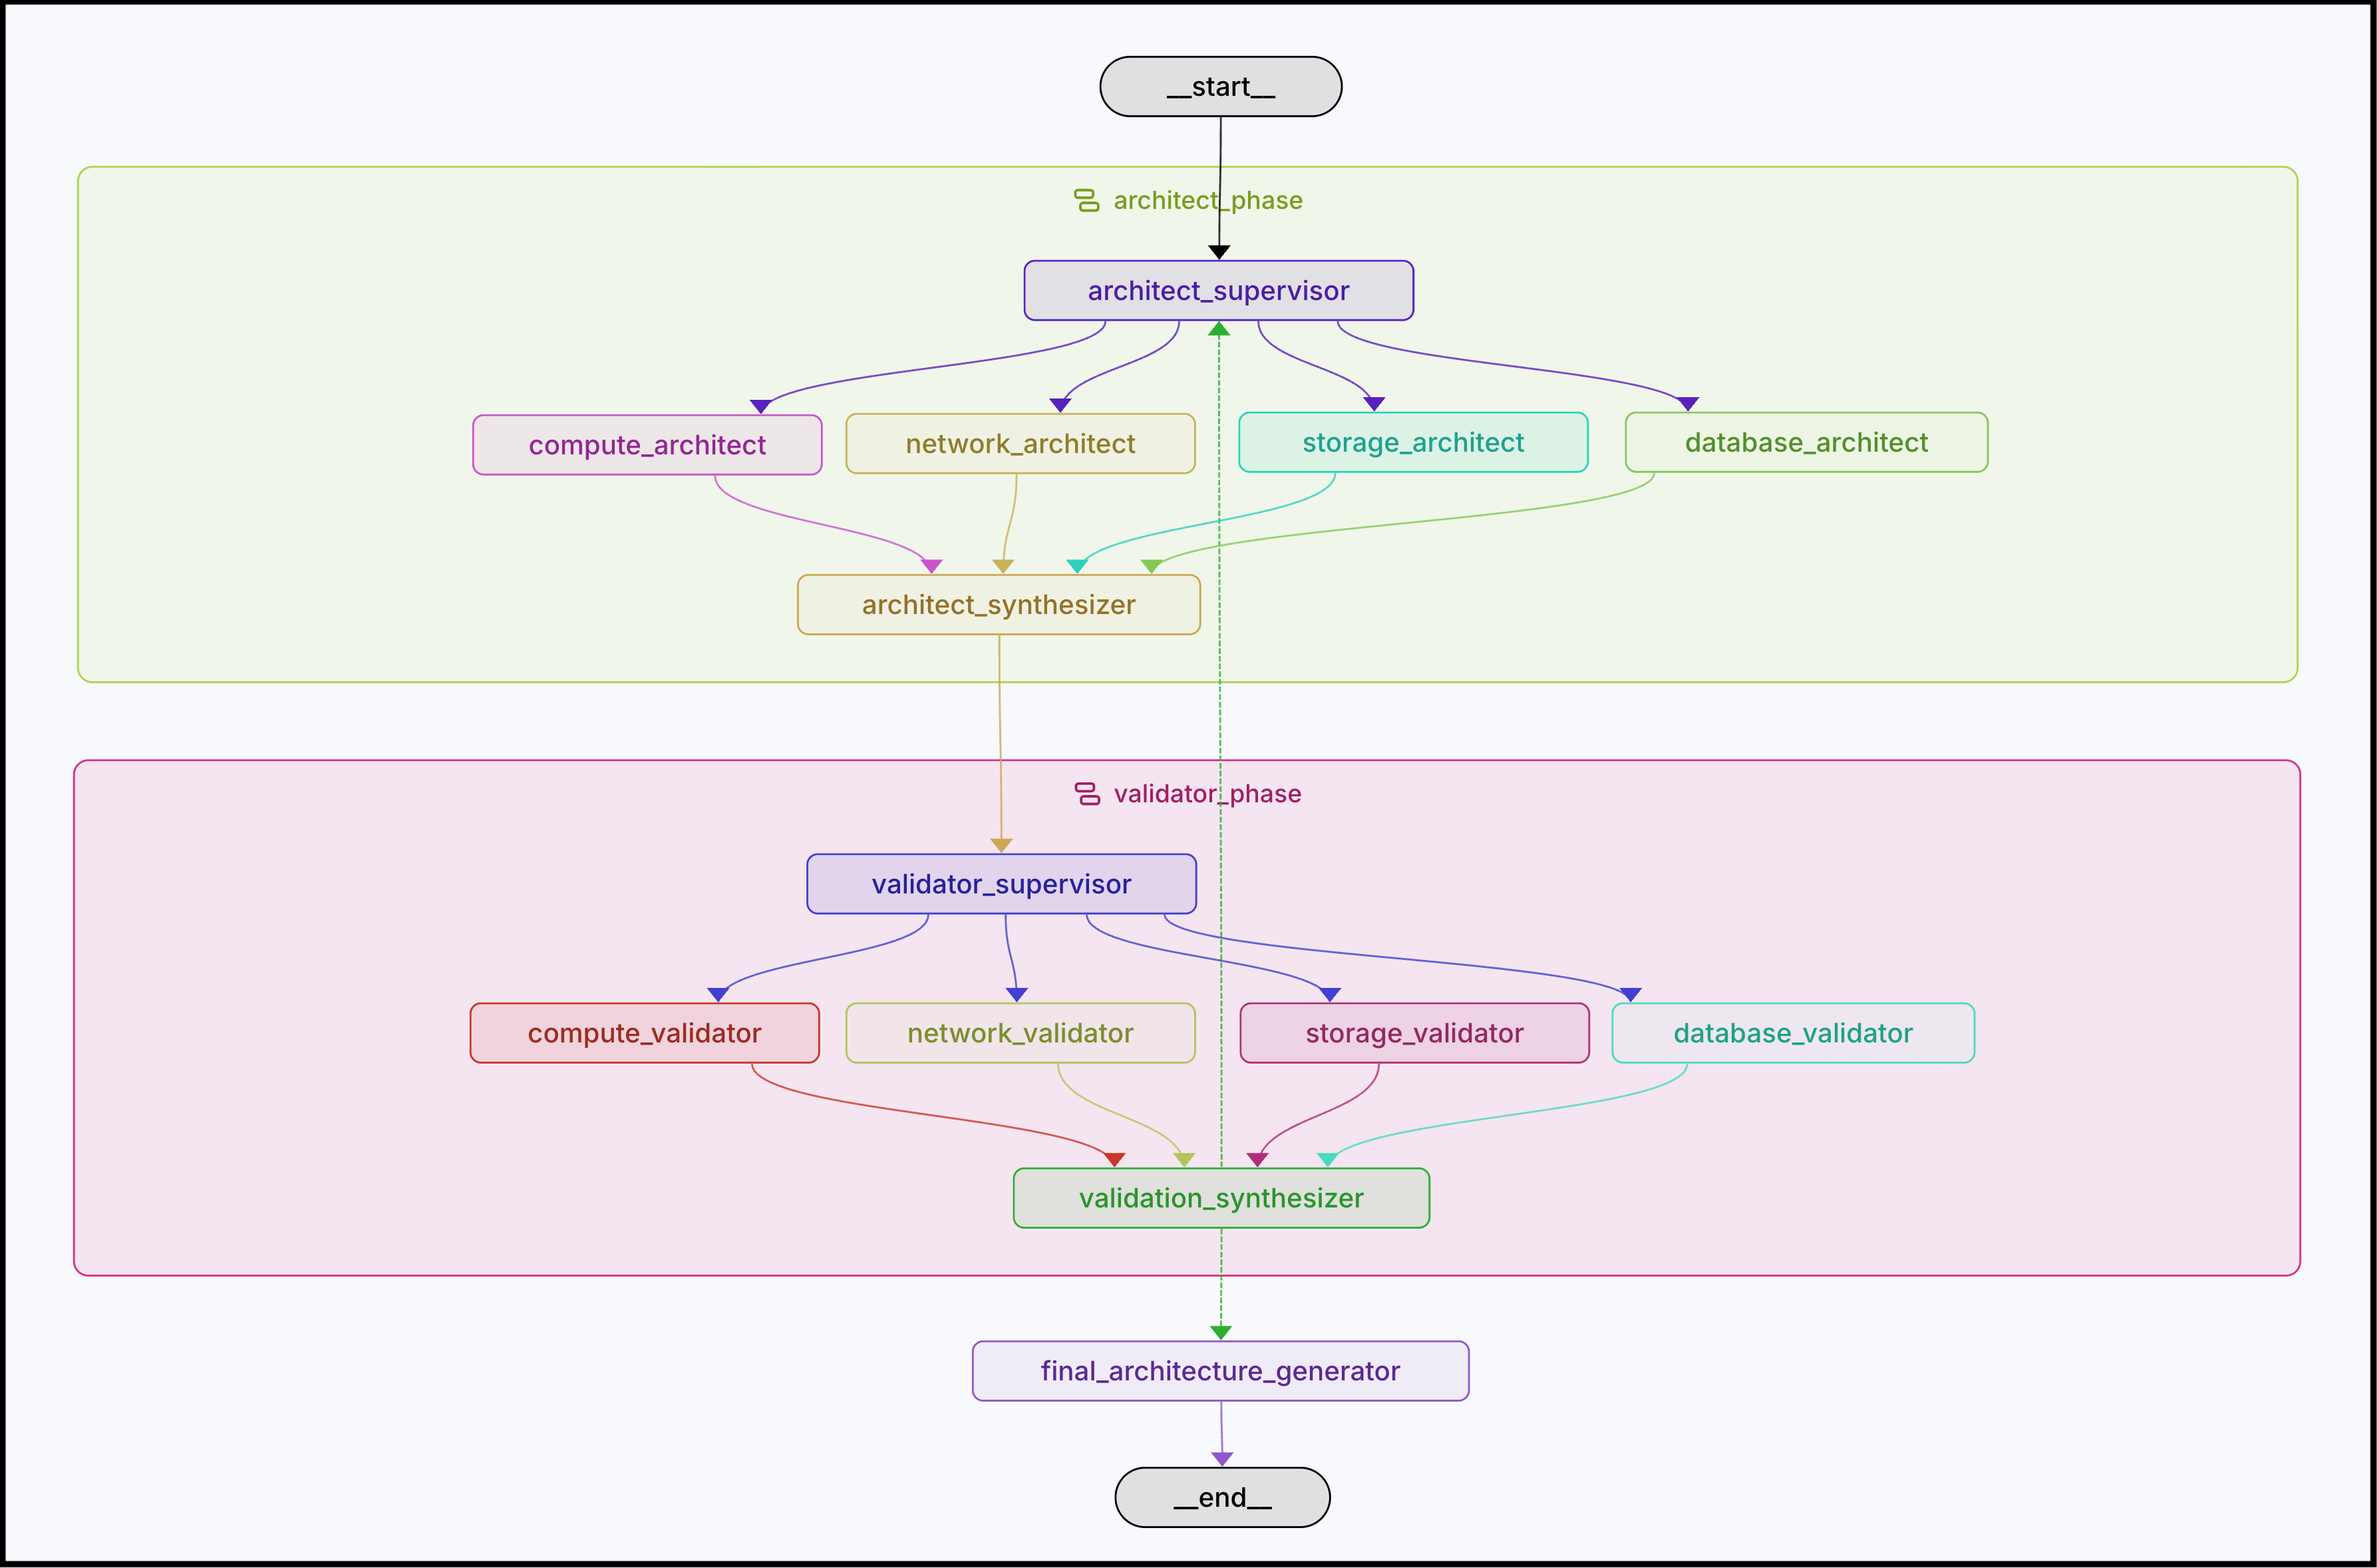
\includegraphics[width=1.05\textwidth, height=0.55\textheight]{./figures/LangGraphStudioGraph.png}
\caption{Agent framework graph generated by LangGraph Studio.}
\label{fig:langgraph}
\end{figure}

\subsection{Graph Topology and Subgraph Composition}

The top-level graph is assembled via subgraph composition. Rather than defining all nodes inline, the implementation composes two independently compiled \texttt{StateGraph} subgraphs \texttt{architect\_phase} and \texttt{validator\_phase} and adds them as single nodes in the parent graph. Each subgraph encapsulates its own  fan-out/fan-in wiring (supervisor $\rightarrow$ four parallel domain agents $\rightarrow$ synthesizer), a pattern conceptually analogous to the MapReduce paradigm~\cite{dean2008mapreduce} from distributed data processing, and is self-contained. Adding a new processing phase (such as cost estimation or compliance checking) requires inserting one node and two edges in the parent graph without touching either existing subgraph.


The architect subgraph connects \texttt{architect\_supervisor} to all four domain architect nodes (\texttt{compute\_architect}, \texttt{network\_architect}, \texttt{storage\_architect}, \texttt{database\_architect}) in parallel, then fans in all four to \texttt{architect\_synthesizer}. The validator subgraph follows the identical pattern with validator counterparts. LangGraph automatically parallelises the four domain agents in each subgraph because they share the same predecessor and successor with no inter-agent data dependencies.

\subsection{Architect Supervisor Agent}

Implementing the query decomposition design described in Chapter~3 (Phase~1), a \texttt{RuntimeContext} is passed during the graph-building stage. On the first iteration the supervisor decomposes the user problem into a \texttt{TaskDecomposition} Pydantic model containing one \texttt{DomainTask} per domain along with global goals and constraints validated via LangChain's \texttt{with\_structured\_output(TaskDecomposition)} binding. This guarantees that downstream agents always receive typed, parseable JSON rather than free-form text.

On subsequent iterations the supervisor reads the \texttt{validation\_feedback} list and \texttt{validation\_summary} string left by the previous validator phase, and incorporates them into its system prompt so that revised task descriptions directly address identified factual errors. Before returning its state update, the supervisor explicitly resets \texttt{validation\_feedback}, \texttt{architecture\_components}, and \texttt{proposed\_architecture} to empty structures, ensuring that parallel domain agents write into a clean slate rather than accumulating stale data from earlier cycles. The supervisor uses the reasoning-tier LLM (default \texttt{gpt-5.4}) and applies exponential backoff retry logic with up to a configurable number of attempts for transient API failures.

\subsection{Domain Architect Agents}

A LangGraph node function is defined for each of the four architectural domains. Each node function:

\begin{enumerate}
    \item Retrieves its \texttt{DomainTask} from the state field.
    \item Constructs a system prompt that incorporates the provider's representative service list for that domain, the task description, requirements, and expected deliverables.
    \item Invokes the execution-tier LLM (default \texttt{gpt-5.4-mini}) inside the bounded tool-calling loop. The loop dispatches outstanding tool calls to either the \texttt{web\_search} tool (Google Serper API) or the \texttt{rag\_search} tool (ChromaDB), appends tool result messages to the conversation context, and re-invokes the LLM. The loop terminates when the LLM produces a response with no further tool calls, or when the per-agent iteration threshold (default 3 rounds).
    \item Extracts the final content string and assigns it to the corresponding domain specific segment of shared state.
\end{enumerate}


\subsection{Architect Synthesizer}

Implementing Phase~3 from Chapter~3, the \texttt{architect\_synthesizer} acts as the fan-in node for the architect subgraph. It receives the complete \texttt{architecture\_components} dictionary assembled from all four parallel domain agents via the \texttt{merge\_dicts} reducer (described in Section~\ref{sec:state_management}) and instructs the reasoning-tier LLM to produce a unified architecture narrative. The synthesiser output is stored in shared state fields and forms the input to the validator phase.

\subsection{Validator Supervisor and Domain Validators}

As designed in Chapter~3 (Phase~4), the \texttt{validator\_supervisor} inspects the proposed architecture components and produces a \texttt{ValidationDecomposition}: a list of \texttt{ValidationTask} objects specifying, for each active domain, which cloud services to scrutinise and which validation focus to apply (e.g.\ configuration correctness, security best practices, or cross-service compatibility). The per-domain validation checklists from the \texttt{ProviderMeta} registry (Section~\ref{sec:provider_meta}) are embedded in the validator system prompts, ensuring consistent evaluation criteria regardless of which model is executing.

Domain validators (\texttt{compute\_validator}, \texttt{network\_validator}, \texttt{storage\_validator}, \texttt{database\_validator}) follow the same bounded tool-calling loop as domain architects, but are bound exclusively to the \texttt{rag\_search} tool. All validation feedback is therefore grounded in the pre-embedded official documentation corpus, not in open-internet search results.

\subsection{Validation Synthesizer and Iteration Routing}

The \texttt{validation\_synthesizer} aggregates the per-domain validator outputs stored in \texttt{validation\_feedback} and consolidates them into a shared state. It sets the \texttt{factual\_errors\_exist} boolean to \texttt{True} if any domain reports factual inconsistencies. The \texttt{iteration\_condition} function then applies the following decision logic:

\begin{itemize}
    \item If the current iteration count is below \texttt{min\_iterations}, return \texttt{"iterate"} unconditionally to enforce a minimum number of refinement passes.
    \item If \texttt{factual\_errors\_exist} is \texttt{True} and the count is below \texttt{max\_iterations}, return \texttt{"iterate"} to trigger corrective re-generation.
    \item If the count has reached \texttt{max\_iterations}, return \texttt{"finish"} as a hard stop to avoid an infinite loop.
    \item Otherwise return \texttt{"finish"}: validation passed and the minimum has been met.
\end{itemize}

This implements the Evaluator-Optimizer feedback loop designed in Chapter~3 (Phase~5), with the routing logic encoded in the graph topology rather than in any explicit loop construct.

\subsection{Final Architecture Generation}

Following the design described in Chapter~3 (Phase~6), once the iteration condition routes to \texttt{"finish"}, the \texttt{final\_architecture\_generator} node compiles the converged state into the deployment-ready output document. The key implementation detail is the injection of the active provider's \texttt{iac\_resource\_hints} field---which maps each architecture domain to canonical Terraform or CloudFormation resource type identifiers (e.g.\ \texttt{aws\_instance}, \texttt{aws\_lambda\_function})---into the IaC sections of the document. The completed document is stored in the \texttt{final\_architecture} state field and constitutes the primary artefact returned to the user interface.

\section{State Management}
\label{sec:state_management}

The LangGraph \texttt{State} is defined as a Python \texttt{TypedDict}, with every field annotated with a custom reducer function via \texttt{Annotated[T, reducer]}. When multiple nodes write partial state updates concurrently, LangGraph calls the appropriate reducer to merge them into a single consistent state. The five reducer functions and their roles are:

\begin{itemize}
    \item \textbf{\texttt{merge\_dicts}:} Applied to \texttt{architecture\_components}, \texttt{architecture\_domain\_tasks}, and \texttt{proposed\_architecture}. When the four parallel domain agents each return a single-key dict (e.g.\ \texttt{\{"compute": \{...\}\}} and \texttt{\{"network": \{...\}\}}), \texttt{merge\_dicts} performs a deep merge into a unified dict keyed by domain name. This enables genuine parallel fan-out: no coordination or locking is required between domain agents.
    \item \textbf{\texttt{last\_value}:} Applied to scalar fields such as \texttt{user\_problem}, \texttt{iteration\_count}, \texttt{architecture\_summary}, \texttt{reasoning\_model}, and \texttt{execution\_model}. The most recent write unconditionally overwrites the previous value.
    \item \textbf{\texttt{or\_reducer}:} Applied to \texttt{design\_flaws\_exist}. Once any domain validator sets this flag to \texttt{True} within an iteration, it remains \texttt{True} for the rest of that cycle, ensuring the supervisor is made aware of any design flaw even if other validators pass.
    \item \textbf{\texttt{overwrite\_bool}:} Applied to \texttt{factual\_errors\_exist}. Unlike \texttt{or\_reducer}, this permits an explicit reset: the architect supervisor clears the flag to \texttt{False} at the start of each new iteration so that validators assess the freshly generated architecture rather than inheriting the previous cycle's error state.
    \item \textbf{\texttt{validation\_feedback\_reducer}:} Applied to the \texttt{validation\_feedback} list. It performs domain-aware deduplication: when a validator re-runs for the same domain in a subsequent iteration, its new entry replaces the stale domain entry rather than appending a duplicate. An empty list emitted mid-run by the supervisor signals an explicit reset, discarding all previous feedback before new validator results accumulate.
\end{itemize}

\section{Model Selection Mechanism}

The model catalog defines nine selectable LLMs across three providers, each represented as a frozen dataclass carrying a canonical identifier, a display name, a provider tag (\texttt{"openai"}, \texttt{"anthropic"}, or \texttt{"google"}), a tier label (\texttt{"reasoning"} or \texttt{"execution"}), and a brief description. The current catalog includes three OpenAI GPT-5.4-family models, three Anthropic Claude 4.6-family models, and three Google Gemini 3.1/2.5-family models.

The model selection function resolves the provider from the catalog and instantiates the appropriate LangChain chat class, \texttt{ChatOpenAI}, \texttt{ChatAnthropic}, or \texttt{ChatGoogleGenerativeAI} at a fixed temperature of 0.1 for deterministic outputs.

By default, the system uses \texttt{gpt-5.4} as the reasoning-tier model (supervisors and synthesisers) and \texttt{gpt-5.4-mini} as the execution-tier model (domain architects and validators), reflecting the cost-quality trade-off discussed in Chapter~3 (Section~3.4).

\section{Interactive User Interface}

The frontend is a Next.js 15 application that communicates with the LangGraph server through the LangGraph SDK streaming API. The UI is organised around five primary React components and a central orchestration hook.

\begin{itemize}
    \item \textbf{WorkflowGraph:} A React Flow~\cite{reactflow2024} canvas that renders the full agent pipeline as an interactive directed graph. Custom node types (agent, tool, decision, start, end) display real-time execution status (idle, active, completed) using coloured ring indicators. The \texttt{useRunOrchestration} hook drives these updates by mapping backend node identifiers received over Server-Sent Events (SSE) to UI node.
    \item \textbf{SidebarNavigator:} The left sidebar exposes navigation across four views---AWS architecture, Azure architecture, side-by-side comparison, and debate mode and a collapsible model selection panel. The panel renders separate dropdowns for the reasoning and execution tiers; each list groups models by provider (OpenAI, Anthropic, Google).
    \item \textbf{CompareView:} A side-by-side layout that renders the AWS and Azure architecture summaries produced from the same problem statement, enabling direct service-level comparison across domains.
    \item \textbf{IaCGenerationPanel:} Displays Infrastructure-as-Code stubs for the generated architecture.
    \item \textbf{CopilotSidebar:} A conversational interface backed by the streaming run API. Architects submit a natural-language problem statement and receive streamed output as the agent graph executes, with individual domain outputs appearing progressively.
\end{itemize}

\section{Evaluation Infrastructure}

\subsection{Benchmark Scenarios}

A set of benchmark problems drawn from public AWS reference architecture blog posts represent a diverse range of real-world patterns. Each scenario is stored as a structured JSON file containing a user problem statement, a full reference architecture text (ground truth), a list of expected cloud services, and the domains covered.

\subsection{Runner Variants}
\label{subsec:runner_variants}

Three runner modules implement a controlled ablation study across framework configurations:

\begin{itemize}
    \item \textbf{Baseline - Single Prompt LLM (Version 1):} Invokes a single LLM call with a structured system prompt but no tool access, producing a zero-shot architecture recommendation. This represents the lower bound: the capability a user would obtain by submitting the problem directly to a chat model.
    \item \textbf{Agentic Framework (Version 2):} Builds a minimal \texttt{START $\rightarrow$ architect\_phase $\rightarrow$ END} graph executing the full architect subgraph (supervisor, four parallel domain agents with web search and RAG tools, synthesizer) in a single pass without any validator phase or iteration. This isolates the contribution of multi-agent decomposition and tool-augmented generation.
    \item \textbf{Complete Evaluator Optimiser Loop Framework (Version 3):} Executes the complete graph with configurable \texttt{min\_iterations} and \texttt{max\_iterations}, giving the full Evaluator-Optimizer loop with iterative validation and refinement.
\end{itemize}

For cross-model comparison experiments, the framework runner sets both the reasoning and execution LLM to the same model name, eliminating confounding from tier-asymmetric model assignments and ensuring that differences in scores are attributable solely to the model under test.

\subsection{LLM-as-a-Judge Evaluation}
\label{subsec:judge_rubric}

Each runner's output is scored by an independent judge LLM using a six-dimension rubric aligned with the AWS Well-Architected Framework~\cite{aws2023wellarchitected}:

\begin{enumerate}
    \item \textbf{Completeness} — breadth of coverage across compute, networking, storage, and data management components.
    \item \textbf{Technical Accuracy} — correctness of service configurations and integration patterns based on official platform documentation.
    \item \textbf{Security} — identity and access control with least-privilege principles, encryption (at rest and in transit), and network isolation mechanisms.
    \item \textbf{Scalability} — support for high availability (e.g., multi-zone or multi-region deployment), load balancing, auto-scaling, and caching strategies.
    \item \textbf{Best Practices Alignment} — adherence to generally accepted cloud architecture best practices and design principles.
    \item \textbf{Specificity} — use of concrete service names, parameter values, and configuration details rather than generic recommendations.
\end{enumerate}

The judge is provided with the problem statement, the reference architecture text from the benchmark scenario, and the generated architecture text, and it returns an integer score from 1 to 10 for each dimension together with a brief justification. The total score is the arithmetic mean of the six dimension scores. To avoid self-evaluation bias, the judge model used during the main evaluation run is independent of the models under test; the judge model selection rationale and its impact on scores are discussed in Chapter~5.

\section{Robustness Features}

Several defensive measures are built in to keep the system stable across non-deterministic LLM calls and long multi-iteration runs.

\textbf{Retry logic:} All LLM invocations in synthesizer and supervisor nodes apply exponential backoff (1\,s, 2\,s, 4\,s delays) for up to a configurable number of attempts (default 2 retries, i.e.\ 3 total attempts) before returning a formatted error message rather than crashing the graph.

\textbf{Bounded tool-calling loops:} Domain architect and validator agents enforce a per-agent iteration threshold (default 3 tool-call rounds) and a timeout (default 120\,s) inside the loop. When either limit is reached the agent extracts the best available content from the conversation history, preventing runaway API cost from stuck tool-call chains.

\textbf{Content normalisation:} A helper transparently handles the heterogeneous response formats returned by different LLM providers. Google Gemini models, for example, return \texttt{content} as a list of typed content-part dicts rather than a plain string; \texttt{normalize\_content} flattens both formats to a uniform string before further processing.

\textbf{LangSmith tracing:} LangSmith integration is configurable via environment variables and records full per-node traces including tool inputs, tool outputs, and LLM token counts for post-hoc debugging of non-deterministic execution paths and for monitoring token expenditure across long evaluation runs.

\section{End-to-End Workflow Trace}
\label{sec:workflow_trace}

The following condensed trace illustrates how the implemented Evaluator-Optimizer loop operates on a representative problem statement. It shows concretely how validation feedback propagates across iterations, how the architect subgraph incorporates that feedback, and how the system converges to a deployment-ready architecture. This trace is representative and condensed for clarity; Figures~\ref{fig:ui_workflow} and~\ref{fig:ui_report} are screenshots from a live system run on a comparable problem statement, confirming that the described behaviour is reproduced faithfully by the deployed system.

\begin{verbatim}
Condensed illustrative trace:

Input: "Design a secure, scalable three-tier web library application
        with auto-scaling, CDN, and managed database."

--- Iteration 1 ---
Architect Supervisor: Decomposing problem into 4 domains:
    compute, network, storage, database.
Domain Architects (parallel):
    Compute  -> EC2 ASG behind ALB; multi-AZ (us-east-1a/1b);
                target-tracking auto-scaling on CPU.
    Network  -> CloudFront + WAF (edge); Route 53; VPC with
                public/private/data subnets; NAT Gateways.
    Storage  -> S3 for static assets (CloudFront origin);
                EBS volumes for application tier.
    Database -> Aurora PostgreSQL (Multi-AZ); ElastiCache for
                Redis (session caching); Secrets Manager.
Architect Synthesizer: Merged proposal committed to state.
Validator Supervisor: Dispatching 4 domain validation tasks.
Domain Validators (parallel):
    Compute  -> FAIL: SG inbound rules use CIDR blocks instead of
                      upstream SG-ID references (violates zero-trust
                      networking); ASG scaling thresholds (CPU %,
                      ALB request count) not specified; ELB health
                      check grace period absent.
    Network  -> PASS
    Storage  -> FAIL: EBS volumes not encrypted; S3 bucket policy
                      does not restrict access to CloudFront OAC;
                      no unified KMS CMK across storage services.
    Database -> PASS
Validation Synthesizer: has_errors=True -> routing to Iteration 2.

--- Iteration 2 ---
Architect Supervisor: Re-decomposing with validation feedback context.
Domain Architects (parallel):
    Compute  -> ASG SG inbound rules rewritten to reference ALB SG
                ID only (no CIDR ingress); target-tracking on CPU
                70% and ALB request count 1,000/min; ELB health
                check grace period 300s; data-tier SG references
                app SG ID only.
    Network  -> CloudFront (OAC for S3, ALB as dynamic origin);
                WAF managed rule groups (OWASP, Bot Control);
                NACLs as secondary deny layer; TLS 1.2+; HSTS.
    Storage  -> EBS encrypted with KMS CMK; S3 OAC bucket policy
                restricts direct access; single KMS CMK proposed
                for EBS and S3 (Secrets Manager still uses
                separate key).
    Database -> Aurora Multi-AZ; PITR enabled; ElastiCache
                encryption in-transit and at-rest.
Architect Synthesizer: Updated proposal committed to state.
Domain Validators (parallel):
    Compute  -> PASS
    Network  -> PASS
    Storage  -> FAIL: KMS CMK not unified -- EBS, RDS, ElastiCache,
                      S3, Secrets Manager, and CloudWatch Logs must
                      all reference a single CMK for centralised
                      key governance; separate keys observed.
    Database -> PASS
Validation Synthesizer: has_errors=True -> routing to Iteration 3.

--- Iteration 3 ---
Architect Supervisor: Re-decomposing with updated feedback context.
Domain Architects (parallel):
    Compute  -> No change required; SG chaining and ASG config
                retained from Iteration 2.
    Network  -> No change required.
    Storage  -> Single KMS CMK now governs EBS, RDS (Aurora),
                ElastiCache, S3, Secrets Manager, and CloudWatch
                Logs; CMK key policy scoped to required principals;
                automatic 30-day Secrets Manager rotation retained.
    Database -> Aurora PITR; ElastiCache encryption updated to
                reference unified KMS CMK.
Architect Synthesizer: Updated proposal committed to state.
Domain Validators (parallel):
    Compute  -> PASS    Network  -> PASS
    Storage  -> PASS    Database -> PASS
Validation Synthesizer: has_errors=False -> routing to Final Generator.

--- Final Output ---
Final Architecture Document generated.
Title: Secure, Scalable Three-Tier Web Library Application on AWS
       Production-Ready Architecture - Version 1.0
Design: Defense-in-depth across three tiers (Presentation,
        Application, Data), each across two AZs (us-east-1a/1b).
Key principles enforced:
  Zero-Trust: All SG inbound rules reference upstream SG IDs;
              no CIDR-based ingress; NACLs as secondary layer.
  Encryption: Single KMS CMK governs EBS, Aurora, ElastiCache,
              S3, Secrets Manager, CloudWatch Logs.
  Scalability: ASG target-tracking (CPU 70%, 1,000 req/min);
               Aurora Multi-AZ; ElastiCache cluster mode.
  Operations:  Managed services (Aurora, ElastiCache, S3);
               all five Well-Architected pillars addressed.
\end{verbatim}

The trace confirms that cross-agent validation feedback propagates correctly across loop iterations and that the system converges when all deficiencies are resolved, even when convergence requires more than two passes. In this run, three iterations were needed: compute and storage validators failed in Iteration~1 (CIDR-based SG ingress, unencrypted EBS, absent CloudFront OAC policy), compute and network passed in Iteration~2 but the storage validator raised a further deficiency---KMS key fragmentation across services---requiring a third architect pass to unify all encryption under a single customer-managed CMK. By Iteration~3, all four domain validators returned passing verdicts. The progression from CIDR-based SG rules to full SG-ID chaining, and from per-service encryption keys to a single CMK governing Aurora, ElastiCache, S3, EBS, Secrets Manager, and CloudWatch Logs, are precisely the kind of deployment-critical details that structured iterative validation surfaces and that a single-prompt response would typically omit.

\begin{figure}[htbp]
    \centering
    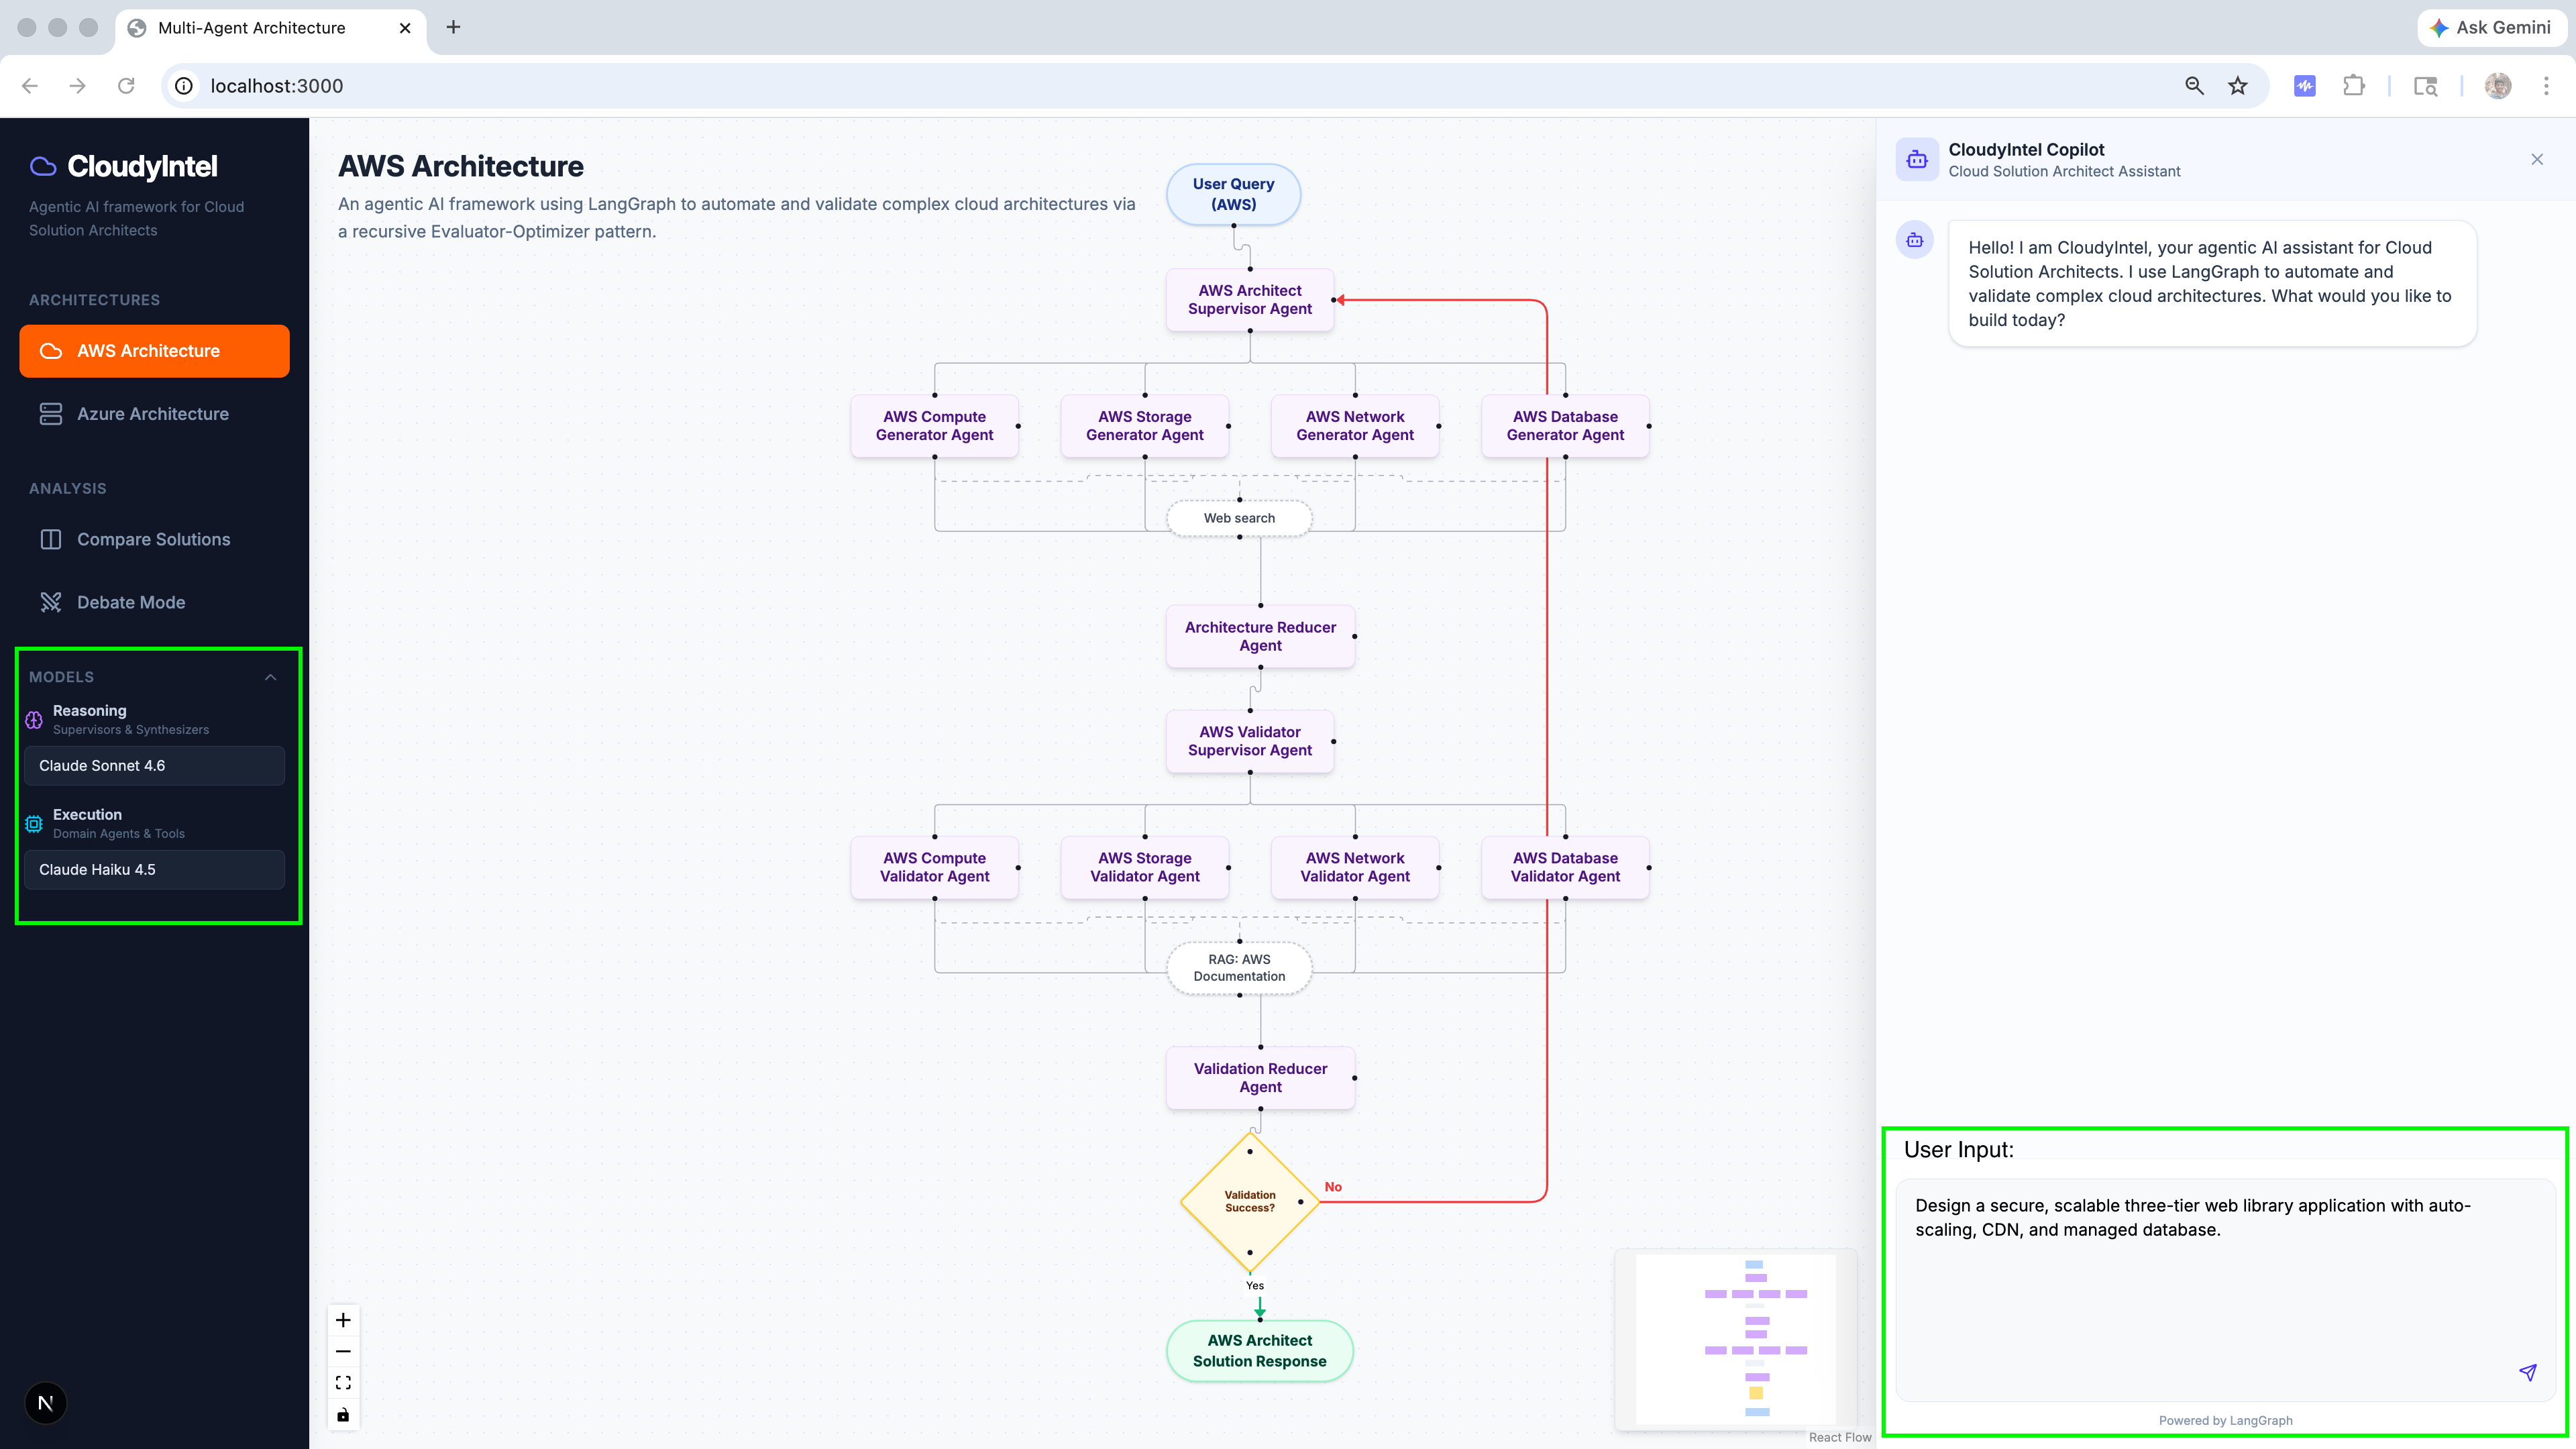
\includegraphics[width=1.0\textwidth]{./figures/ui_workflow_graph.png}
    \caption{The user interface showing the problem statement in the right-hand panel and the dynamic model selection panel on the left, with the reasoning tier set to Claude Sonnet~4.6 and the execution tier set to Claude Haiku~4.5.}
    \label{fig:ui_workflow}
\end{figure}

\begin{figure}[htbp]
    \centering
    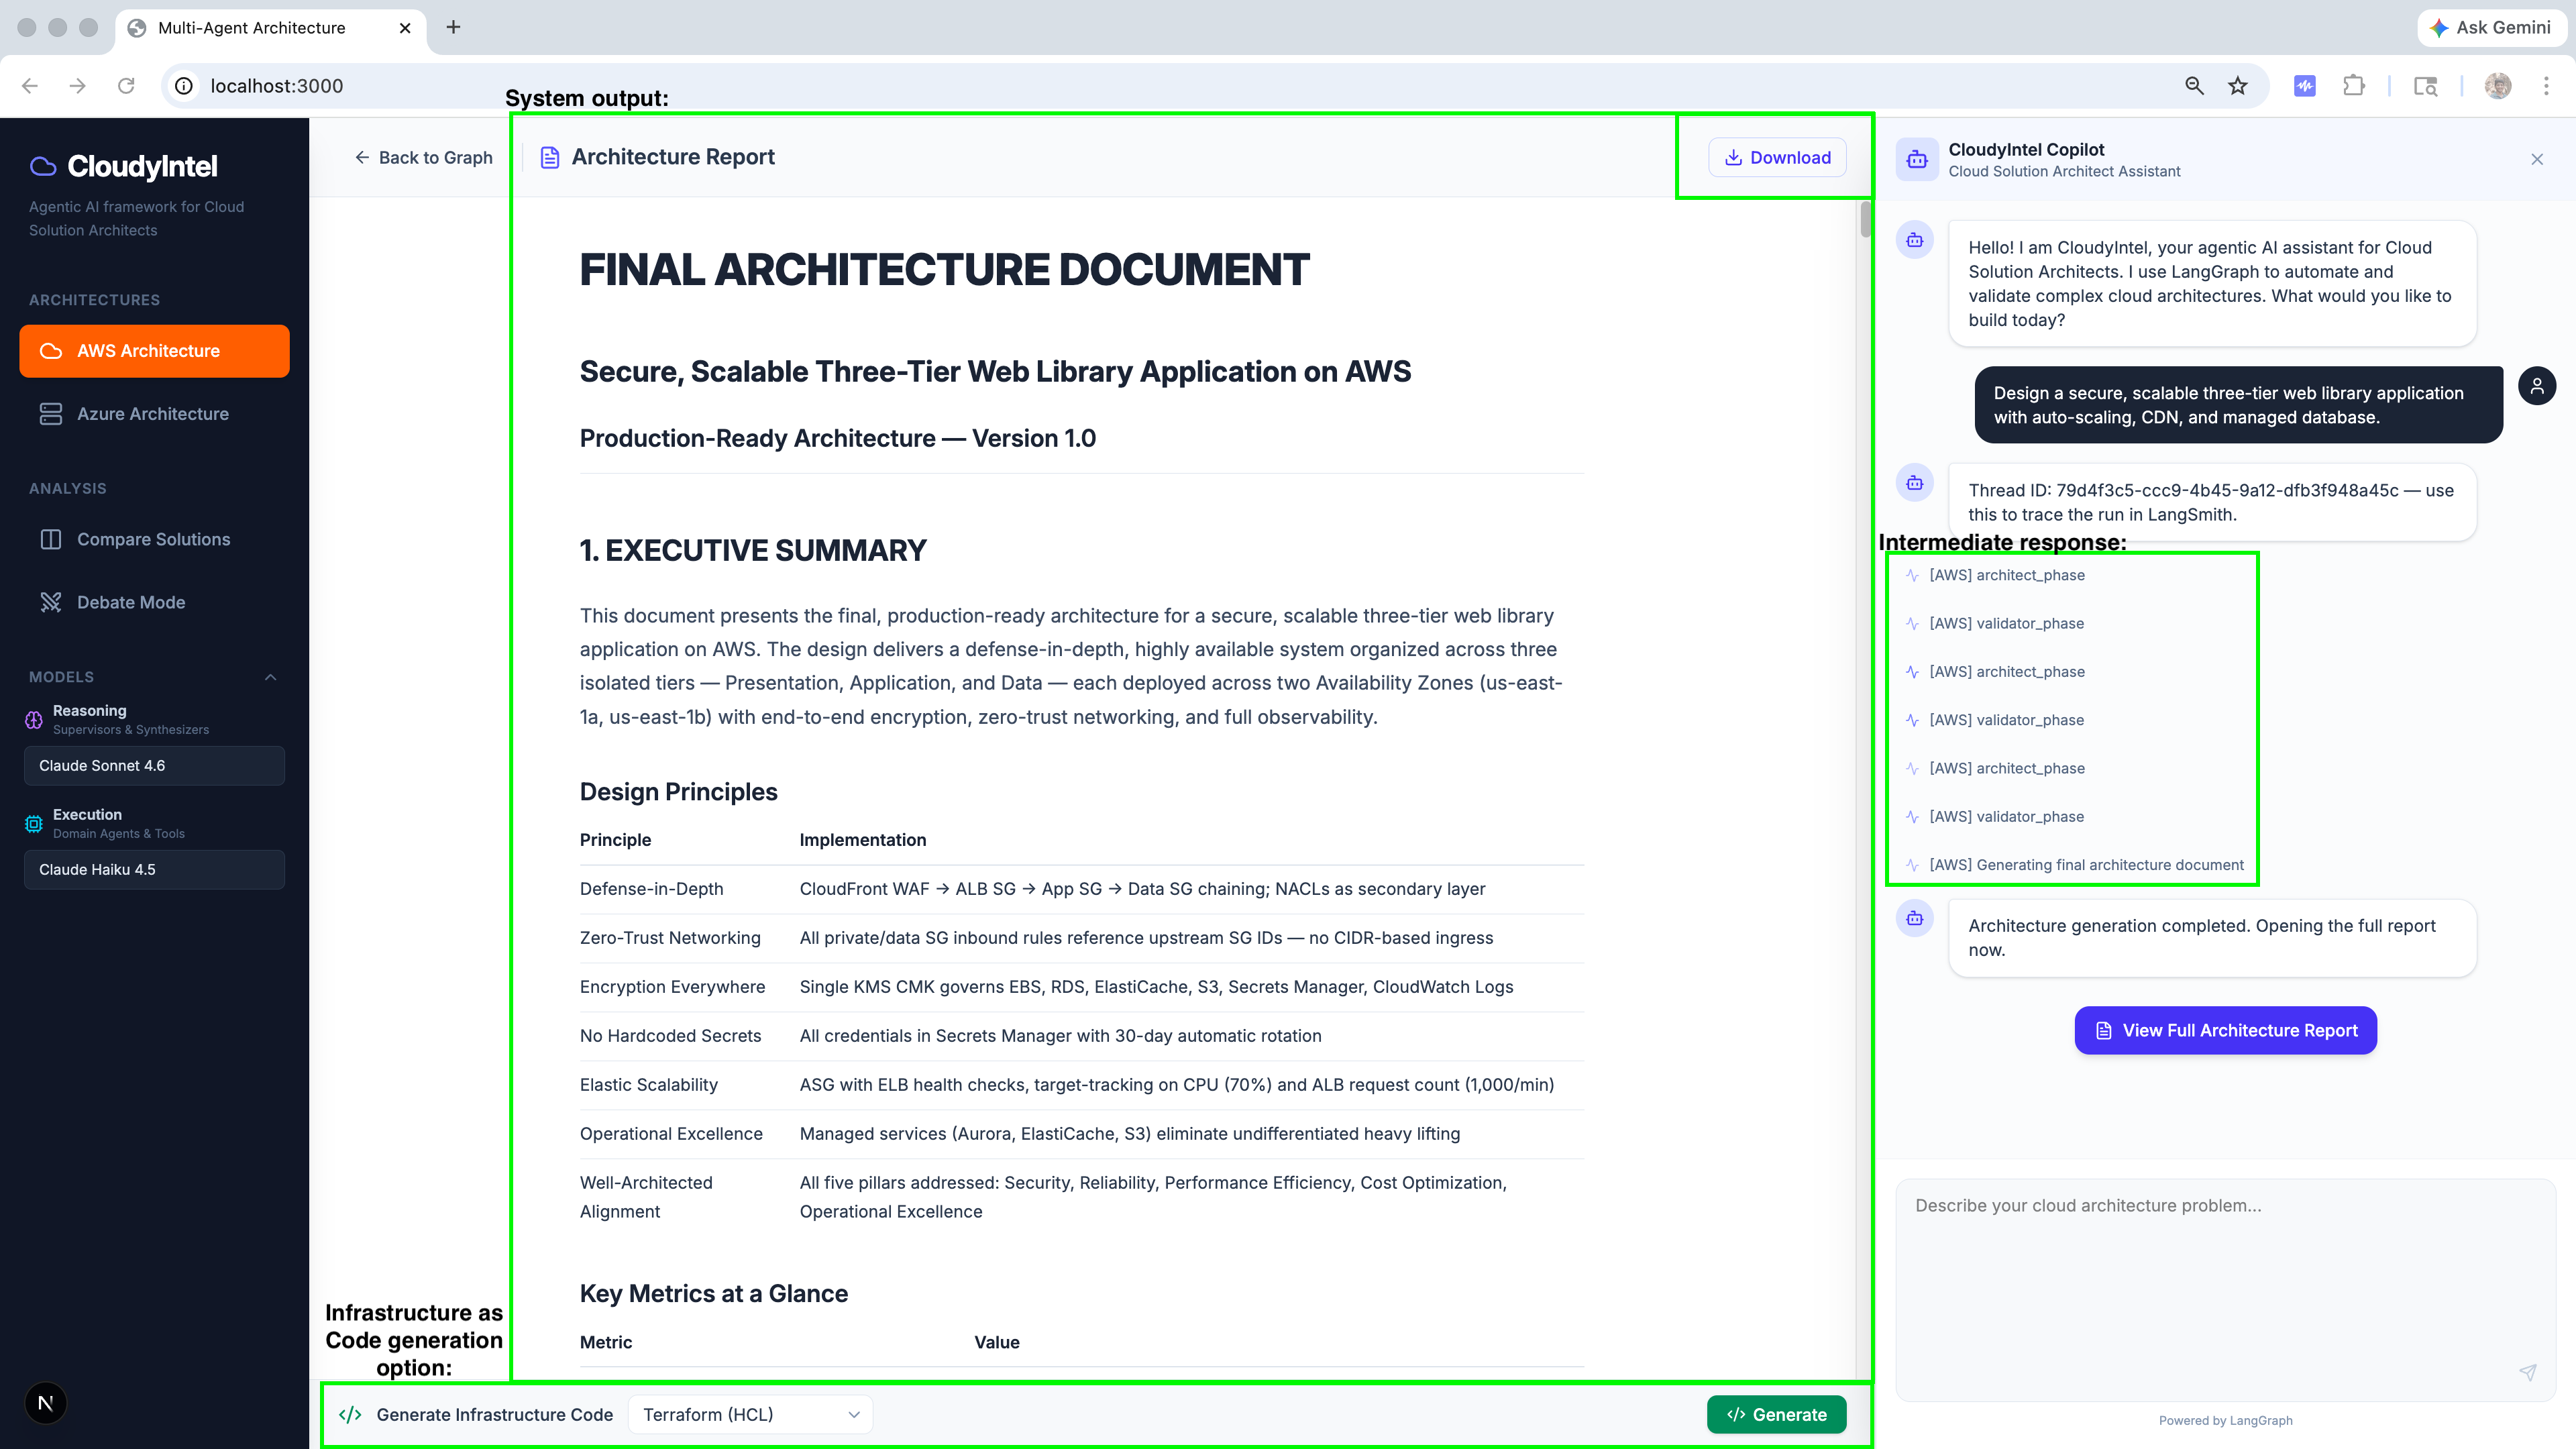
\includegraphics[width=1.0\textwidth]{./figures/ui_architecture_report.png}
    \caption{The generated Final Architecture Document alongside the intermediate response panel, which records three complete \texttt{architect\_phase} $\to$ \texttt{validator\_phase} cycles before the final document is produced, providing direct evidence of multi-iteration convergence in the live system.}
    \label{fig:ui_report}
\end{figure}